% Nejprve uvedeme tridu dokumentu s volbami
\documentclass[bc,female,java,dept456]{diploma}						% jednostranny dokument
\usepackage[czech]{babel}
%\usepackage[cp1250]{inputenc}
\usepackage[utf8]{inputenc}
\usepackage{comment}
\usepackage{graphicx}
\usepackage{url}
\usepackage{longtable}
%\usepackage{dialogue}

\setcounter{secnumdepth}{2}




% Zadame pozadovane vstupy pro generovani titulnich stran.
\Author{Michal Hantl}

\Title{Nástroj pro monitorování chování uživatelů webových aplikací}

\EnglishTitle{A tool for monitoring web application user behaviour}

\SubmissionDate{20. dubna 2011}

\PrintPublicationAgreement{true}




\Thanks{Rád bych na tomto místě poděkoval svým rodičům za podporu během celého studia, panu Ing. Michalovi Radeckému, za vedení během vypracování diplomové práce a své přítelkyni Míše.}





\CzechAbstract{
Cílem práce je vytvoření nástroje, jakožto podpory pro aplikaci a navržení metody získávání informací o chování uživatele webové aplikace. Nebude se jednat o klasický přístup založený na sběru statistických dat anonymních návštěvníků, ale o využití znalosti o konkrétním uživateli, jeho chování, využívání funkcí a služeb webové aplikace.

Výsledkem praktické části je webová aplikace ...
}

\CzechKeywords{webová analytika, chování uživatelů, webová aplikace, diplomová práce}

\EnglishAbstract{
The goal of this thesis is to create a tool to aid web application development and to create a method for gaining knowledge of the web application users' behaviour. It is not the case of usual anonymized data gathering, but make us of the knowledge of concrete user, his behaviour and his usage of web app's functions and services. 
}

\EnglishKeywords{web analytics, user behaviour, web application, master thesis}





% Pridame pouzivane zkratky (pokud nejake pouzivame).
\AddAcronym{GUI}{Grafické uživatelské rozhraní (Graphical User Interface)}
\AddAcronym{HTML}{Jazyk pro vytváření webových stránek (HyperText Markup Language)}







% Zacatek dokumentu
\begin{document}

% Nechame vysazet titulni strany.
\MakeTitlePages

% Asi urcite budeme potrebovat obsah prace.
\tableofcontents
\cleardoublepage	% odstrankujeme, u jednostranneho dokumentu o jednu stranku, u oboustrenneho o dve

% Jsou v praci tabulky? Pokud ano vysazime jejich seznam.
% Pokud ne smazeme nasledujici makro.
%\listoftables
%\cleardoublepage	% odstrankujeme, u jednostranneho dokumentu o jednu stranku, u oboustrenneho o dve

% Jsou v praci obrazky? Pokud ano vysazime jejich seznam.
\listoffigures
\cleardoublepage	% odstrankujeme, u jednostranneho dokumentu o jednu stranku, u oboustrenneho o dve


% Jsou v praci vypisy programu? Pokud ano vysazime jejich seznam.
\lstlistoflistings
\cleardoublepage	% odstrankujeme, u jednostranneho dokumentu o jednu stranku, u oboustrenneho o dve










\section{Úvod}
\label{sec:Uvod}


Tato diplomová práce se zabývá webovou analytikou a novým nástrojem pro analytiku webových aplikací. 

Od vzniku webových stránek se web rozvíjel až do dnešní podoby a webová analytika ho provázela. Čím sofistikovanějšími se webové stránky stávaly, tím důmyslnější způsoby byly nacházeny k analýze uživatelského chování.

Z počátku byly používány nástroje na straně serveru, které pasivně analyzovaly data o návštěvách stránek. Až v polovině dvadesátkých let masivní vývoj webových prohlížečů přesunul sběr dat na stranu klienta, kde umožnil aktivní sběr dat o uživatelském chování přímo na stránce.

Sběr dat na straně klienta umožnil rozvoj jednoduše použitelných nástrojů pro webovou analytiku. Ty však svým způsobem stále kopírují konvenční přístup k analýze návštěvníků.

Současné metody měření a interpretace dat dobře vyhovují jednorázovým účelům jako je měření konverze reklamní kampaně, nebo poskytují průměrné statistiky, jako je top 10 nejnavštěvovanějších stránek na serveru v daném období.

Kromě webových stránek jsou na internetu také webové aplikace. Moderní technologie jako HTML5 se snaží smazat rozdíl mezi desktopovou aplikací a tou webovou. Tento trend potvrzuje i to, že Google připravuje svůj vlastní operační systém, který je výhradně založen na webovém prohlížeči a všechny aplikace poběží v něm.

Možnosti webových aplikací jsou již nyní rozšířeny o podporu audia, videa (včetně manipulace) a zobrazení trojrozměrných objektů pomocí technologie WebGl. 

Někteří i tak budou tvrdit, že webové aplikace se nikdy nebudou moci měřit s desktopovými. To by možná byla pravda, pokud by jistá posvátná hranice mezi internetovým prohlížečem a nativní aplikací nebyla překročena technologií NaCl\footnote{NaCl není jediná technologie, která rozšiřuje možnosti prohlížeče o funkce a ryhlost nativního kódu. V současnosti se k těmto účelům používá Adobe Flash, nebo Microsoft Silverlight. Jde však o první implementaci, která si klade za cíl spouštět nativní kód, nepodléhající proprietární technologii.} - nativním kódem pro webové aplikace. Ano, v budoucnu budeme moci spouštět nativní kód v prohlížeči. Tím končí exkluzivní postavení desktopových aplikací.

\bigskip

S nástupem webových aplikací se mění i požadavky na nástroje webové analytiky. Webová aplikace se od webové stránky liší v několika věcech. Obecně rozdíl mezi stránkou a aplikací je interakce. Do webových aplikací vstupují uživatelská data ať už ve tradiční formě hodnot z formuláře, nebo data, které vznikají samotnou interakcí (například  malování). 

Když tedy uživatel vkládá, nebo vytváří v aplikaci data, je třeba je nějak uložit k tomu, aby mohly být později vyvolána a dalo se s nimi pracovat. Pro tento účel webové aplikace vyžadují způsob, jak unikátně identifikovat uživatele. V praxi to znamená, že se uživatel musí zaregistrovat a potvrdit svou identitu e-mailem\footnote{Stále častější alternativou se stávají identifikační autority jako Facebook, Twitter, nebo OpenId. To umožňuje, že uživatel nemusí vyplňovat email, ani heslo a je přihlášen pomocí jediného kliknutí.}.

Právě to, že je uživatel přihlášen dává nové možnosti vývoje nástrojů pro webobou analytiku. Narozdíl od webových stránek, kde nemůžeme s jistotou určit, zda se jedná o stejného uživatele můžeme podle přihlášení s jistotou tvrdit, že se o jedná o stejného uživatele a víme kterého.

V prostředí, kde je uživatel přihlášen můžeme na data pohlížet zcela jiným způsobem. Vezměme si statistiku počtu návštěv, kterou zpracovává Google Analytics a podává ji hned na hlavní stránce statistik pro daný web. Denní počet návštěv je vypočítán tak, že pokud přijdu na stránku ráno, v poledne a večer, započítá se to jako tři návštěvy. Pro webovou stránku to dává smysl ze dvou důvodů. Zaprvé ze stejného počítače může přijít ráno v poledne a večer úplně jiný člověk a to nelze nijak rozeznat. Zadruhé webové stránky nemají uživatele, ale návštěvníky tudíž dává smysl sledovat návštěvy. 

Na druhé straně jsou aplikace, které mají uživatele a tak dává smysl sledovat používání. Jestli uživatel přijde třikrát denně, nebo jednou a stráví v aplikaci 3x tolik času je hezké vědět, ale není to tak podstatné. Co je podstatné je kolik uživatelů reálně dnes navštívilo aplikaci a kolik v ní strávili času.

Tento rozdíl se nezdá na první pohled až tak markantní. Je třeba si uvědomit, že se jedná o odlišný úhel pohledu a z toho vycházejí odlišné závěry. Například z Google Analytics se dá zjistit, kolik procent návštěv je z mobilních zařízení. 

Řekněme, že mobilní zařízení tvoří 3\% všech návštěv. To není jako mnoho, pravděpodobně neznamená, že budeme urpavovat naši aplikaci speciálně pro mobilní zařázení. Na druhou stranu, pokud máme 85\% uživatelů, kteří používají free účet a 15\% platících\footnote{Freemium model, spočívá v účtech zdarma a placených, které poskytují něco navíc.}, mohou tři procenta znamenat až 20\% platících uživatelů. Pokud máme více, než jeden placený tarif, například basic (\$19), gold (\$49) a platinum (\$199). V takovém případě bude velmi důležité vědět, kolik z našich 3\% je ve kterém tarifu.

\bigskip

Některé věci, které jsem popsal Google Analytics umožňuje. Je pouze na uživateli, aby si svoje Analytics co nejlépe nastavil a svou aplikaci opatřil příslušným nastavením, které umožní sledovat zajímavé údaje o uživateli.

Tento univerzální přístup ovšem znamená, že co si užiavtel sám neudělá, to nemá. Další omezení spočívá v tom, že Analytics zakazuje identifikovat uživatele.

Tato situace mě motivovala k vývoji nástroje, který je výhradně zaměřen na analytiku webových aplikací s důrazem na práci s uživateli. Nejedná se pouze o přesnění výsledků, jde o to zaměřit se na zákazníky a nikoliv na průměrná čísla.












\section{Webová analytika}

Tato kapitola popisuje vznik webové analytiky a způsoby sběru a intepretace dat v obecné rovině. 



\subsection{Historie}

Jak již bylo řečeno v úvodu, dnešní nástoje v podstatě kopírují způsob interpretace dat a proto je vhodné nastínit historii webové analytiky. Je proto vhodné se chvíli pozastavit nad tím, jak to všechno začalo.

Na začátku devadesátých let došlo ke zrození WWW stránek[reference]. Uživatelé tehdy prohlíželi statické stránky a pokaždé, když si nějakou prohlédli, vznikl záznam v logovacím souboru, takzvaný "hit". Počet hitů se stal ukazatelem úspěšnosti webový stránek.

V roce devadesát čtyři vznikl grafický webový prohlížeč s názvem Mosaic[reference]. Díky jeho snadné instalaci a srozumitelnému uživatelskému rozhraní se web otevřel široké veřejnosti. Tento prohlížeč byl později přejmenován na Netscape a v roce 1995 ho používalo 80\% uživatelů internetu.

V roce devadesát pět znikl Analog - nástroj pro analýzu logovacích souborů. Jeho autor Stephen Turner ho poskytoval zdarma jako freeware pro několik platform. Jednalo se o první sofistikovaný nástroj pro analýzu a zobrazení návštěvnosti webových stránek.

\bigskip

\begin{lstlisting}[label=src:Plain,caption=Ukázka záznamu z logovacího souboru ve formátu RFC931]
10.20.30.40 - - [26/Apr/2000:00:23:48 -0400] "GET /index.html HTTP/1.0" 200 6248 "http://www.jafsoft.com/asctortf/" "Mozilla/4.05 (Macintosh; I; PPC)"
10.20.30.40 - - [26/Apr/2000:00:23:48 -0400] "GET /background.gif HTTP/1.0" 200 4005 "http://www.example.org/" "Mozilla/4.05 (Macintosh; I; PPC)"
\end{lstlisting}

\bigskip

Logovací soubor obsahuje jden řádek pro každou návštěvu stránky, nebo souboru na serveru. Nástroj pro analýzu logovacích souborů z toho pak dokáže zjistit kolik měl server návštěv každý den, z kolika unikátních IP adres, které stránky jsou nejnavštěvovanější a kolik bylo přenesených dat.

\begin{comment}
The data collection became unusable with the advent of search engines and their robots, proxies servers to surf anonymously, allocation of dynamic IP addresses by ISPs and cached content techniques. All these developments have rendered the use of log files inappropriate to analyze user behavior. The data contained in log files were indeed biased and unique visitor identification almost impossible. 
\end{comment}

\begin{figure}[h]
	\centering
	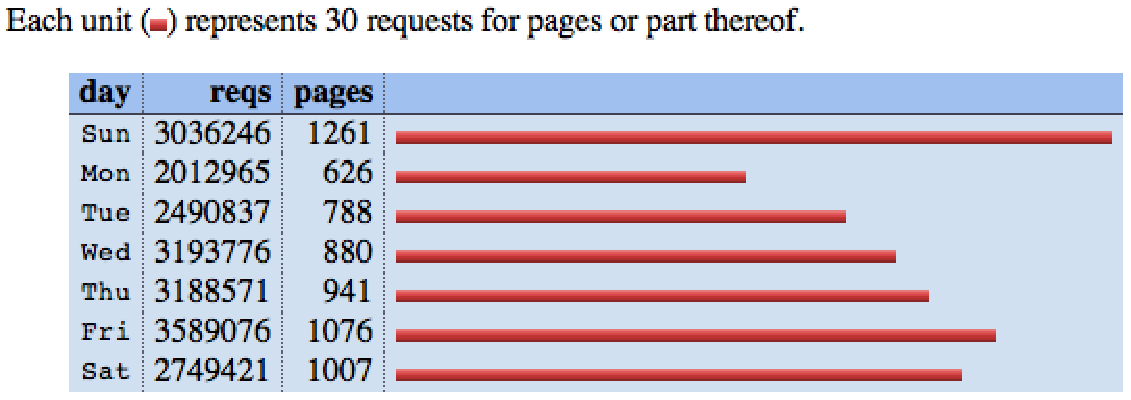
\includegraphics[width=14cm]{img/analog_daily.pdf}
	\caption{Analog - denní návštěvnost}
	\label{analog_daily}
\end{figure}


V roce 1996 byl v obou nejpoužívanějších prohlížečích\footnote{V roce 1996 měl Netscape Navigator zhruba 80\% podíl a Internet Explorer 14\%} k dispozici JavaScript. 

Tvůrce webových stránek na každou stránku umístil kód, který mu vygeneroval poskytovatel měřícího nástroje. 


Tento postup se zásadně liší od analýzy logových souborů. Místo statické analýzy zaznamenaných dat na straně serveru tento přístup data dynamicky sbírá na straně klienta.

Tento průlom umožnil použtití třetích stran pro sběr i vyhodnocení dat a tak dal vzniknout prvním online nástrojům pro webovou analytiku. V různých obměnách se tato technika používá dodnes.

V roce 2005 koupila společnost Google analytický systém Urchin on Demand a ještě v témž roce ho poskytla zdarma široké veřejnosti jako webovou aplikaci pod názvem Google Aanlytics. Pro obrovský zájem byl tento produkt zpřístupněn pouze omezenému počtu uživatelů. Od října roku 2006 byly znovu otevřeny volné registrace a dodnes se jedná o nejpoužívanější systém pro webovou analytiku.

\bigskip

S nástupem sociálních médií a chytrých mobilních zařízení dochází k nárůstu času, který uživatelé tráví na internetu. Poměrně k tomuto nárůstu se zvyšují investice do internetových stránek a webových aplikací. 

Na jedné straně je snaha dostat nové uživatele na svou stránku, to se dociluje například pomocí optimalizace pro vyhledávače, reklamních bannerů, nebo PPC reklamy\footnote{PPC - Pay per click, platba za proklik (cena prokliku je určena pomocí aukce).}. V tomto případě slouží webová analytika k měření efektivity jednotlivých kampaní a k jejich následné optimalizaci.

Na druhé je snaha pracovat s uživateli, které už webová stránka, nebo aplikace má. Zde je snaha identifikovat problémy a optimalizavat uživatelskou zkušenost. V obou případech je to webová analytika, která nám umožňuje získat přehled, optimalzovat a vyhodnotit návratnost investic.

{\bf Nástroj, kterým se tato práce zabývá je primárně zaměřen na práci s uživateli}.









\subsection{Sběr dat}

Podstatou webové analytiky je sběr a interpretace dat. Jak již bylo řečeno, sběr dat se za dobu existence webu vyvinul z pasivní formy analýzy logových souborů na serveru do dnešní - aktivního sběru dat na straně uživatele třetí stranou.

Tato kapitola popisuje popisuje používané způsoby sběru dat s důrazem na to, jaké informace z nich získáváme, jaké další informace z nich můžeme vyčíst a jaké způsoby vizualizace se běžně vyskytují.





\subsubsection{Analýza dat z logovacích souborů}

Webové servery zaznamenávají zobrazení stránek do takzvaných logovacích souborů. Jedná se o soubory, ve kterých každý řádek představuje záznam o jednom zobrazení stránky, nebo například obrázku.

Když na začátku devadesátých let vznikl web, provozovatelé serverů si uvědomili, že tyto soubory umožňují získat informace o popularitě jejich stránek a tak začali měřit počet zobrazení, takzvaných "hitů". V té době se vyskytovaly většinou pouze dlouhé stránky bez obrázků nebo odkazů, takže počet zobrazení postačoval potřebám provozovatelů.

\bigskip

\begin{lstlisting}[label=src:Plain,caption=Formát logovacího souboru dle RFC931]
127.0.0.1 - frank [10/Oct/2000:13:55:36 -0700] "GET /apache_pb.gif HTTP/1.0" 200 2326
\end{lstlisting}

\bigskip

\begin{longtable}{ lp{9cm} }
  \verb!127.0.0.1! & IP adresa návštěvníka. Počet unikátních IP adres byl původně používán jako hrubý odhad počtu uživatelů. \\ \bigskip
  \verb!-! & pomlčka \\ \bigskip
  \verb!frank! & Uživatelské jméno. Tento údaj je přítomen v případě se stránka používá HTTP autentifikaci. To platí pro stránky s omezením přístupu pro uzavřenou skupinu lidí a tudíž u náhodného návštěvníka stránky tento údaj nenajdeme. V takovém případě se místo uživatelského jména zaznamená pomlčka. \\ \bigskip
  \verb!10/Oct/2000! & Datum návštěvy. \\ \bigskip
  \verb!13:55:36! & Čas návštěvy, vztahuje se k časové zóně na serveru. \\ \bigskip  
  
  \verb!-0700! & Časová zóna. \\ \bigskip
  \verb!GET /apache_pb.gif! & Požadavek a verze HTTP protokolu \\ \bigskip
  \verb!HTTP/1.0! & Požadavek HTTP protokolu. GET je základním požadavkem, který signalizuje, že uživatel požaduje nějaký obsah. Další používaný požadavek je například POST, který se používá pro odeslání formuláře na server.  \\ \bigskip
  
  \verb!200! & Kód odpovědi. Kód 200 znamená vše v pořádku. Obvyklé a pro webovou analytiku také zajímavé jsou 404 - stránka nenalezena, 500 - problém na serveru, nebo 303 - přesměrování stránky. \\ \bigskip
  \verb!2326! & Délka odpovědi v bajtech. Sledování této veličiny spolu s počtem návštěv umožňuje identifikovat, který obsah nejvíce zatěžuje internetové připojení daného serveru.
\end{longtable}






\begin{comment}
This is the IP address of the client (remote host) which made the request to the server. If HostnameLookups is set to On, then the server will try to determine the hostname and log it in place of the IP address. However, this configuration is not recommended since it can significantly slow the server. Instead, it is best to use a log post-processor such as logresolve to determine the hostnames. The IP address reported here is not necessarily the address of the machine at which the user is sitting. If a proxy server exists between the user and the server, this address will be the address of the proxy, rather than the originating machine.
- (%l)
The "hyphen" in the output indicates that the requested piece of information is not available. In this case, the information that is not available is the RFC 1413 identity of the client determined by identd on the clients machine. This information is highly unreliable and should almost never be used except on tightly controlled internal networks. Apache httpd will not even attempt to determine this information unless IdentityCheck is set to On.
frank (%u)
This is the userid of the person requesting the document as determined by HTTP authentication. The same value is typically provided to CGI scripts in the REMOTE_USER environment variable. If the status code for the request (see below) is 401, then this value should not be trusted because the user is not yet authenticated. If the document is not password protected, this entry will be "-" just like the previous one.

[10/Oct/2000:13:55:36 -0700] (%t)
The time that the server finished processing the request. The format is:
[day/month/year:hour:minute:second zone]
day = 2*digit
month = 3*letter
year = 4*digit
hour = 2*digit
minute = 2*digit
second = 2*digit
zone = (`+' | `-') 4*digit
It is possible to have the time displayed in another format by specifying %{format}t in the log format string, where format is as in strftime(3) from the C standard library.
"GET /apache_pb.gif HTTP/1.0" (\"%r\")
The request line from the client is given in double quotes. The request line contains a great deal of useful information. First, the method used by the client is GET. Second, the client requested the resource /apache_pb.gif, and third, the client used the protocol HTTP/1.0. It is also possible to log one or more parts of the request line independently. For example, the format string "%m %U%q %H" will log the method, path, query-string, and protocol, resulting in exactly the same output as "%r".
200 (%>s)
This is the status code that the server sends back to the client. This information is very valuable, because it reveals whether the request resulted in a successful response (codes beginning in 2), a redirection (codes beginning in 3), an error caused by the client (codes beginning in 4), or an error in the server (codes beginning in 5). The full list of possible status codes can be found in the HTTP specification (RFC2616 section 10).
2326 (%b)
The last entry indicates the size of the object returned to the client, not including the response headers. If no content was returned to the client, this value will be "-". To log "0" for no content, use %B instead.
\end{comment}

Jak web rostl, tak i jeho složitost a z jednoduchých stránek bez obrázků se staly různě provázené stránky s odkazy a obrázky. S vzůrstající složitostí internetových stránek se i nástroje pro analýzu logovacích souborů stávaly sofistikovanější a začaly na sebe nabalovat další možnosti.

Pole zaznamenávaných dat sbíraných v logovacích souborech byl rozšířen o další informace HTTP protokolu, kterými se zabývá další část kapitoly. Samotný formát je z hlediska anlaytiky vedlejší a není není již nutno ho rozebírat.





  
\subsubsection{Informace získané pomocí HTTP protokolu}

Prohlížení webových stránek na internetu je zajišťěno pomocí HTTP protokolu. HTTP je zkratka pro Hyper Text Tranfer Protokol, neboli protokol pro výměnu hypertextů (hypertextových stránek). Je to způsob jak webový prohlížeč komunikuje s webovým serverem.

Pomocí HTTP protokolu poskytuje prohlížeč informace o uživateli tak, aby webový server mohl co nejlépe vyhovět požadavku.

Formátem HTTP protokolu se na tomto místě není třeba zabývat. Stačí vědět, že obsahuje podstatné jsou informace, které se používají ve webové analytice. Pro názornost je uveden příklad HTTP požadavku a některých základních informací, které obsahuje.

\bigskip

\begin{lstlisting}[label=src:Plain,caption=Ukázka HTTP požadavku]
GET /dumprequest HTTP/1.1
Host: djce.org.uk
Connection: keep-alive
Accept: application/xml,application/xhtml+xml,text/html;q=0.9,text/plain;q=0.8,image/png,*/*;q=0.5
User-Agent: Mozilla/5.0 (X11; U; Linux i686; en-US) AppleWebKit/534.16 (KHTML, like Gecko) Chrome/10.0.634.0 Safari/534.16
Accept-Encoding: gzip,deflate,sdch
Accept-Language: cs-CZ,cs;q=0.8
Accept-Charset: windows-1250,utf-8;q=0.7,*;q=0.3
\end{lstlisting}

Nyní je třeba si říct, jaké informace můžeme získat a k čemu se dají využít. Jsou to:

\subsubsection{Požadovaná stránka}

Udává o kterou stránku je zájem. Tento údaj se v nejjednodušším příkladě používá k určení popularity jednotlivých stránek na webovém serveru. Z hlediska toho, jak jsou dnešní webové stránky strukturovány, dá se předpokládat, že čím hlouběji je stránka zanořená ve stromové struktuře webu, tím toto číslo bude menší. Například:

\begin{verbatim}
--+ Hlavní stránka 			(150 návštěv)
  |--+ Podstránka 1			( 50 návštěv)
  |  \-- Pod-pod stránka	( 10 návštěv)
  \--- Podstránka 2			( 50 návštěv)
\end{verbatim}

Tato informace má různý význam v různých kontextech. Uvažujme informační server na kterém každý den vyjde několik článků v různých kategoriích. Hlavní stránka klade největší důraz na nejnovější články a v postranním panelu obsahuje odkazy na jednotlivé kategorie článků.

\begin{verbatim}
--+ Hlavní stránka informačního serveru		
  |-- 1. Nejnovější článek
  |-- 2. Nejnovější článek		
  |-- 3. Nejnovější článek	
  ...
  |-- Kategorie článků A
  \-- Kategorie článků B  
\end{verbatim}

Pro kategorie znamená počet zobrazení popularitu jednotlivých kategorií. Tento údaj by měl být odpovídat počtu zobrazení článků v jednotlivých kategoriích a měl by se porovnávat k počtu zobrazení dalších kategorií. Například v případě že poměr návštěv kategorie vaření je velký ale poměr přečtení článků o vaření je malý, může to například znamenat, že kategorie je zajímavá ale neobsahuje tak zajímavé články.

Pro stránku, která představuje článek je počet zobrazení ukazatelem toho, jak je článek populární. S touto informaci je se dále pracuje a interpretuje se. Je třeba dát do kotextu:
\begin{itemize}
  \item{které webové stránky na daný článek odkázaly}
  \item{kolik vzniklo ke článku komentářů}
  \item{kolik lidí kliklo na článek z hlavní stránky}
  \item{jaký je u článku titulek a obrázek, jestli článek}
\end{itemize}


V kontextu webové aplikace se může jednat o údaj, který udává nejpoužívanější sadu funkcí. Následující příklad toto demonstruje na zjednodušené administraci E-shopu.

\begin{verbatim}
--+ Administrace E-shopu
  |-+ Objednávky
  | |-- nevyřízené objednávky
  | |-- vyřízené objednávky
  | \-- hledat objednávky
  |-- Zboží
  \-- Nastavení  
\end{verbatim}

V této fiktivní administraci E-shopu jsou tři hlavní podstránky - Objednávky, Zboží a Nastavení. V tomto případě počet zobrazení jednotlivých kategorií umožňuje zjistit (zhruba), jak často je pracováno s objednávkami v poměru se zbožím a nastavením.

V každém případu počet zobrazených stránek představuje trochu jinou informaci a je třeba je interpretovat v podle typu měřené stránky (případně aplikace) a toho jak ji uživatelé používají.

\subsubsection{Referrer}

Údaj refferer je stránka, ze které uživatel přišel. Dá se tedy zjistit, odkud uživatelé na stránku přicházejí a spočítat nejčastější zdroje návštěv.

Ještě zajímavější využití této informace je v případě, že uživatel přišel z vyhledávače. Pak se dá z referreru zjistit, jakou frázi uživatel vyhledával a jaké vyhledávače dominují v počtu přivedených zákazníků.

\subsubsection{Query string}

V query string části adresy se nacházejí údaje, které modifikují obsah stránky. Je to část adresy stránky za otazníkem a není povinná. Například, pokud zadáte "web analytics" do hledání v Google, bude adresa stránky vypadat následovně:

\begin{verbatim}
www.google.com/search?sourceid=chrome&ie=UTF-8&q=web+analytics
\end{verbatim}

\begin{tabular}{ll}
	Část adresy & Význam \\	\hline \smallskip
	znak "?" & začátek query string \\ \smallskip
	znak "\&" & odděluje dvojice klíče a hodnoty \\ \smallskip
	sourceid=chrome & prohlížeč je Google Chrome \\ \smallskip
	ie=UTF-8 & požadujeme výslednou stránku v UTF-8 \\ \smallskip
	q=web+analytics & vyhledávaný dotaz je "web analytics"
\end{tabular}

\bigskip

Stejný princip se používá například když uživatel listuje produkty v elektronickém obchodě. V část adresy bude obsahovat informaci o tom, na které stránce se nachází.

Významné využití je například ve zjišťování, co zákazníci v elektronickém obchodě hledají a jaké fráze při tom používají. Zajímavé je také kolik zákazníků vyhledávání používá a jak často.

%%\subsubsection{Akceptovaný jazyk}

Pokud má uživatel v operačním systému nastavený jazyk češtinu, HTTP požadavek říká serveru, že preferuje českou verzi obsahu. Tato informace je zajímavá především pro servery s velkou návštěvností, které plánují přidat jazykovou mutaci.


%\subsubsection{Prohlížeče a jejich verze}

Podíly jednotlivých prohlížečů se mění podle zaměření stránek a zeměpisných podmínek. Na stránkách o technologiích Microsoftu se dá očekávat vyšší podíl Internet Exploreru\footnote{Internetový prohlížeč od Miscrosoftu}, na stránkách o vaření se zase mohou objevovat vyšší podíly starých prohlížečů. Každý web by měl fungovat pod většinou prohlížečů, pokud se však jedná o stránku o nových technologiích, kde převažují moderní prohlížeče, může se majitel rozhodnout o využití moderních vlatností těhto prohlížečů.

Na druhou stranu na stránkách s vysokým podílem starých prohlížečů se dá očekávat, že uživatelé stránky zobrazují na starých počítačích a tak je třeba tomu přizpůsobit obsah stránky, aby bylo prohlížení bezproblémové a plynulé.

%%\subsubsection{Možnosti HTTP a JavaScripu}

Většina těhto informací se dá zjistit jak pomocí JavaScriptu na straně klienta, tak pomocí HTTP protokolu na straně serveru.

V sekci ~\ref{sec:moznosti} je tabulka porovnání toho, co je možno měřit oběma metodami. Všechny následující informace vznikají přímo v prohlížeči a jediný způsob, jak se dají měřit je JavaScriptem.


%\subsubsection{Události v prohlížeči}

Událostí je myšlen klik na tlačítko, psaní do textového pole, skrolování na stránce, dokonce i pohyb myší a změna velikosti prohlížeče. Jedná se o interakci uživatele se stránkou - ta probíhá v rámci prohlížeče na straně uživatele a tudíž není ji možno měřit jinak, než na straně uživatele.

K sběru dat na straně uživatele se používá JavaScript, který v určitých intervalech posílá tyto informace na server třetí strany, která je vyhodnocuje a smysluplně zobrazuje.

Tato čás popisuje jednotlivé události a jaké mají využití ve webové analytice.






Klikání myší je na stránce způsobuje přechod na jinou stránku, spuštění nějaké funkce, nebo nic, pokud uživatel klikl v místě, kterému není přiřazená žádná funkce.

\begin{comment}
Událost kliku na stránce poskytuje tyto informace:

\begin{itemize}
	\item pozici myši na stránce v okamžiku kliku
	\item objeckt, na který bylo kliknuto
	\item stav kláves ctrl, shift a alt v okamžiku kliku
	\item tlačítko kliknutí (levé, pravé, prostřední a kombinace)
\end{itemize}
\end{comment}

{\bf Interakce s aktiviními prvky} na stránce. V dnešní době obsahují stránky aktivní prvky, například fotoalba umožňují větší náhled obrázku bez nutnostni přejít na novou stránku. Protože tento náhled nezpůsobí zobrazení nové stránky, nevznikne ani nový záznam návštěvy stránky a většina nástrojů pro webovou analytiku tuto skutečnost nezaznamenávají.

{\bf Odchozí odkazy}. Odkaz, který vede na stránku na jiném serveru, říkáme takovému odkazu odchozí. Provozovatele serveru může zajímat, kam z jeho stránky návštěvníci odcházejí. Autora článku zajímá, které odkazy z jeho článku jsou nejzajímavější pro jeho čtenáře.

Sledování {\bf odkazů na soubory} umožňuje získat podobný přehled jako odchozí odkazy. Zatímco analýza logových souborů sleduje stahování souborů na serveru, sběr dat na straně klienta tuto informaci získá, když uživatel klikne na odkaz.

Ze všech kliků na stránce se navíc sestavují takzvané heatmapy\footnote{Heatmapy zobrazují TODO, viz sekce TODO}





Pohyb myši na stránce není kritický faktor, který je třeba sledovat na všech webech jako například kliky myší. Samy o sobě nemají velkou vypovídají hodnotu, existují však nástroje, které je těhto informací dokážou využít.

Agregace pohybů myší se využívá ke konstrukci heatmap. Účel heatmap je graficky znázornit, kterým částem webové stránky se dostává nejvíce pozornosti, ty se zobrazují teplými barvami (žlutá, červená), místa kterým se nedostává pozornost jsou naopak laděny do studeých barev (zelená, modrá). Více o heatmapách v sekci\ref{sec:Heatmaps}


Druhým zcela pdlišným způsobem využití znalosti o pohybu myši je mouse-tracking. Tato technika kombinuje sledování kliků a pohybů myši a tak pořizuje záznam o uživatelově činnosti na stránce. Jedná se o velmi specifickou techniku, která se používá k testování stránek ještě dřív, než se uvolní na veřejnost, nebo k optimalizaci těch částí stránky, kde dochází ke sledované konverzi\footnote{Konverze TODO}. Příklad apliakce mouse-trackingu ke sledování konverze je například v proces dokončení objednávky elektronickém obchodě.





Události používání kláves se používá nejčastěji ve spojení s mouse-trackingem (viz Pohyb myši) k testování uživatelské zkušenosti, nebo k optimalizalizaci objednávkových formulářů v podobných situacích.

Některé webové stránky kladou velký důraz na přístupnost a umožňují uživateli se navigovat pomocí klávesových zkratek. V takovém případě by měli měřit i používání těchto zkratek a případně je upravit tak, aby byla navigace na jejich webu co nejjednodušší.




Událost skrolování stránky nastává když uživatel posouvá stránku nahoru a dolů, případně doprava nebo doleva. Podle  posuvu stránky v určitých intervalech se dá usuzovat, že uživatel stránky čte, nebo pouze prohlíží. Podle délky čtení a toho, jestli se uživatel dostal až na konec článku se dá určit, jestli článek dočetl.

V kombinací s velikostí vnítřní části okna prohlížeče se dá přesně uričit, na kterou část stránky se uživatel dívá. Toho se například využívá k vykreslení heatmapy, která kolik času uživatelé věnují jednotlivým částem stránky. 



{\bf Odchod ze stránky} je událost, která je spuštěna když uživatel přechází na jinou stránku, nebo zavírá okno se stránkou. 

Tato událost se používá k vypočtení tzv "bounce rate". Bounce rate je procento uživatelů, kteří na stránku přijdou a hned zase odejdou. Takové chování se dá očekávat například, když uživatel něco hledá ve vyhledávači, prohlédne si a vzápětí odchází, protože na první pohled stránka neobsahuje informace, které hledal.

Bounce rate je třeba chápat v kontextu s tím, odkud uživatel přichází. Měl by se odlišovat podle zdroje, odkud návštěvník přišel. Například návštěvníci z vyhledávače budou mít odlišný bounce rate, než návštěvníci z odkazujících článků, reklamy, nebo ti, kteří přímo napíší adresu stránky do adresního řádku.


Rozlišení obrazovky, stejně jako používaný prohlížeč je informace která vypovídá o návštěvníkovi a zařízení, které používá. Starší monitory mají například poměr stran 4:3, novější zase 16:9 a 16:10. Stejně tak se dá usuzovat, že u nízkých rozlišení moderních úhlopříček se bude jednat o netbooky a notebooky. Nejvyšší rozlišení mají nejmodernější dvaceti sedmi palcové monitory, a ještě větší rozlišení jako je 3200x1200 znamená, že má uživatel dva monitory, konkrétně s rozlišením 1920x1200 a 1280x1024.


Velikost viewportu TODO


(zobrazení stránek, jako analýza logů)
 


  
  
\subsubsection{Možnosti logfile analýzy a page-taggingu}
\label{sec:moznosti}

\begin{comment}
\begin{tabular}{ l c c }
informace 				& logfile analýza & page-tagging \\ 
\hline
objem přenesených dat	& $\bullet$ & $\circ$ \\
stránka 				& $\bullet$	& $\bullet$ \\
referrer				& $\bullet$	& $\bullet$ \\
query string			& $\bullet$	& $\bullet$ \\
jazyk					& $\bullet$	& $\bullet$ \\
prohlížeč				& $\bullet$	& $\bullet$ \\
odchozí odkazy			& $\circ$	& $\bullet$ \\
doba na stránce			& $\circ$	& $\bullet$ \\
opuštění stránky		& $\circ$	& $\bullet$ \\
rozlišení obrazovky		& $\circ$	& $\bullet$ \\
velikost viewportu		& $\circ$	& $\bullet$ \\
zobrazená část stránky	& $\circ$	& $\bullet$ \\

\end{tabular}
\end{comment}
\bigskip
  

\subsection{Interpretace dat}

Přidaná hodnota analytických nástrojů spočívá v interpretaci nasbíraných dat. Většina údajů, podle kterých se orientujeme vzniká kombinací několika událostí, nebo informací.

Díky cookies\footnote{Do tzv. Cookie je možno uložit uživateli zhruba 4096 znaků a internetový prohlížeč se o tuto hodnotu stará.} je možné sledovat návštěvnka stránky. Při první návštěvě se návštěvníkovi uloží do cookies jeho unikátní identifikátor a lze tak při příští návštěvě identifikovat, že se jedná o stejného návštěvníka. Označování návštěvníků umožňuje zjistit například počet unikátních návštěvníků. Přesto, že někteří uživatelé si Cookie ručně mažou, většina to nedělá a počet unikátních návštěvníků se dá pokládat za relativně přesný.

Označování uživatelů umožňuje také sledovat počet návštěv. Pokud uživatel stráví pět minut prohlížením stránek, zavře stránku a pak se za dvě hodiny vrátí, vyhodnocuje se to jako dvě návštěvy.

Dlouhodobé opakování návštěv označujeme jako loajalitu návštěvníků. Stránky, které mají tuto hodnotu vysokou mají stabilní bázi návštěvníků, kteří si tam zvykli pravidelně chodit. Tato hodnota je důležitá pro informační servery, elektronické obchody, blogy, fóra a komunitní stránky.

{\bf Doba strávená na stránce}

\bigskip

Podle IP adresy návštěvníků se zjišťuje jejich poloha a zobrazuje se pomocí jednoduché mapy. Na obrázku \ref{img:analytics-map} je ukázka takové mapy, která znázorňuje počet návštěv pro Ameriku. Jendá se o statiskiku pro rozšíření do prohlížeče Google Chrome. Jelikož se jdná o rozšíření pro technické typy, lze usuzovat, že takoví se vyskytují v Kalifornii (tmavě zelená vlevo) a New Yorku.

\begin{figure}[hp]
	\centering
	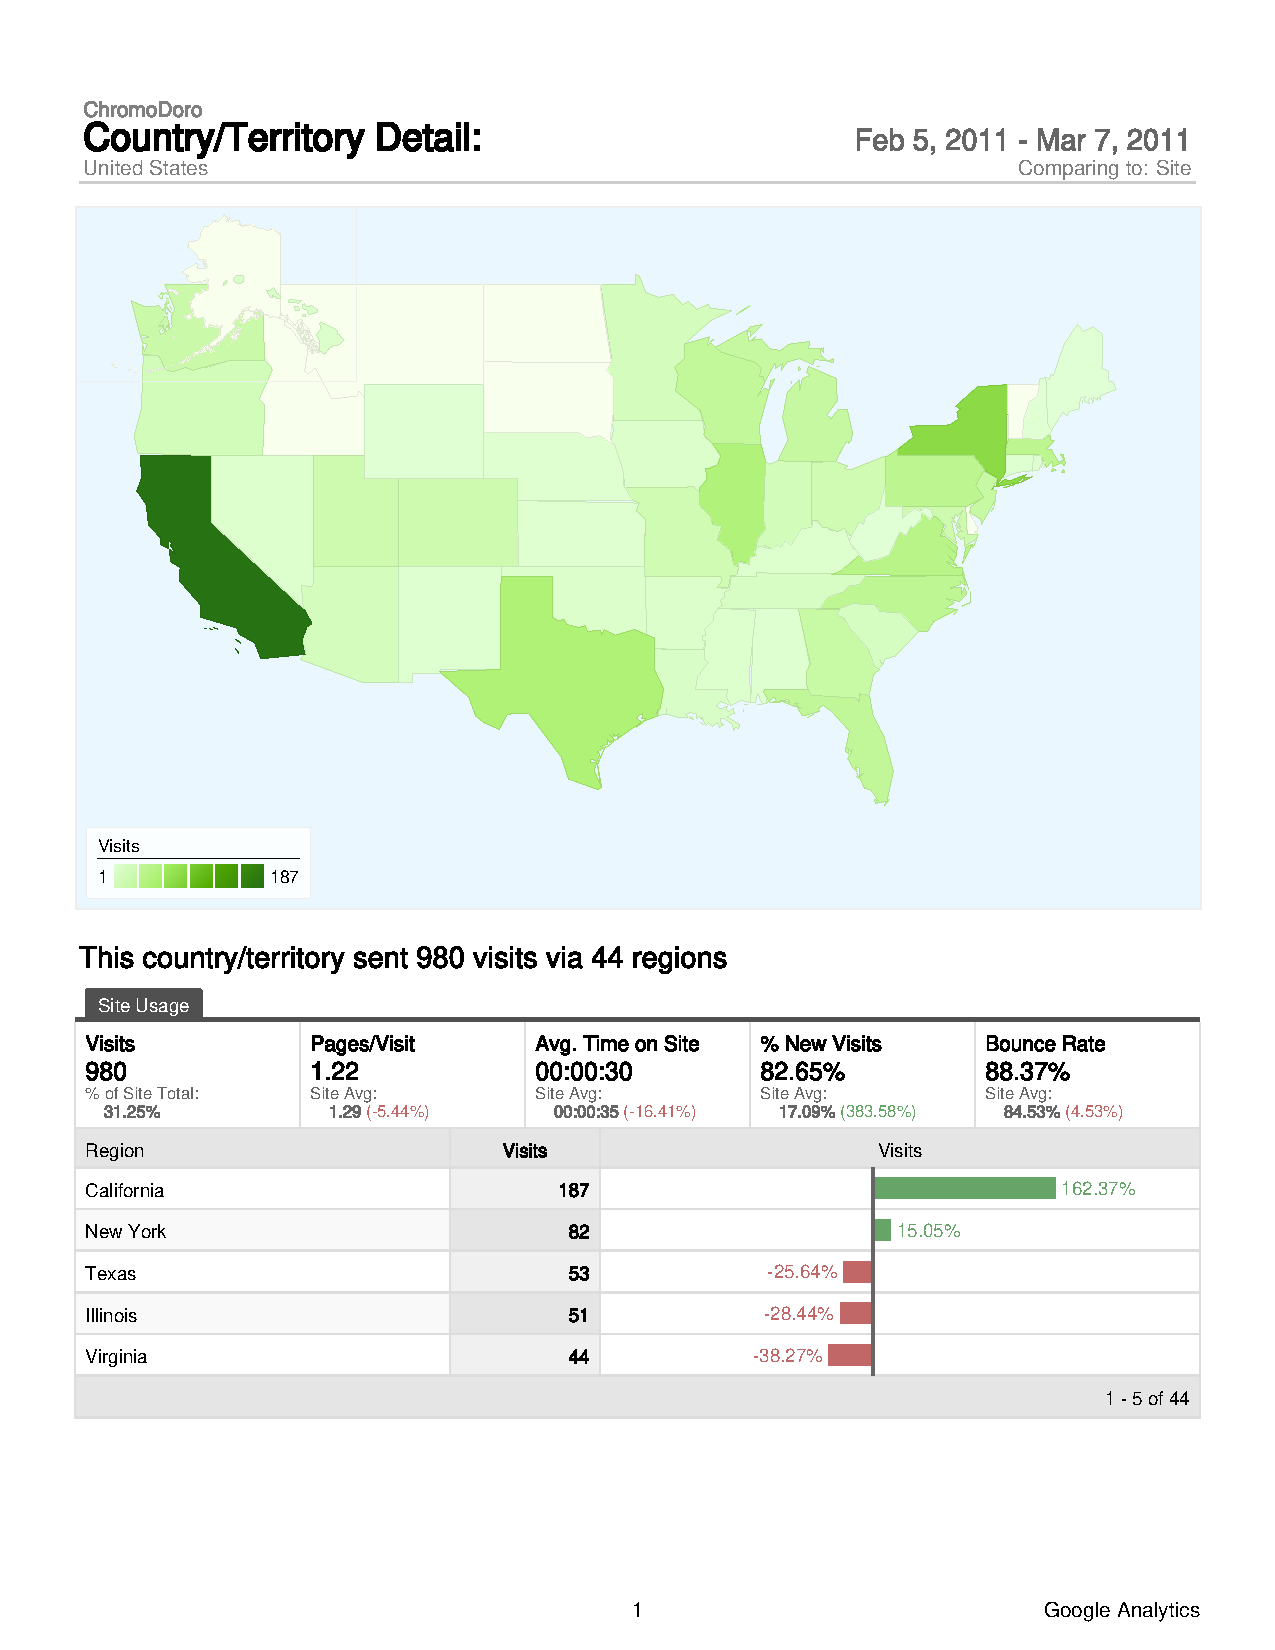
\includegraphics[width=14.25cm]{img/map-analytics.pdf}
	\caption{Google Analytics - návštěvy podle zemí}
	\label{img:analytics-map}
\end{figure}

\bigskip

Na obrázku \ref{img:heatmap-bing-google} je ukázka heatmapy pro stránky výsledků vyhledávačů Google a Bing. Vstupními daty pro vytvoření takových interpretací jsou v ideálním případě data získaná pomocí sledování očních pohybů návštěvníků pomocí speciální kamery. Takovéto testování je možnos provádět pouze v laboratoři a s potřebným vybavením.

Mimo laboratoř je možno takové obrázky vygenerovat z pohybů myší a klikání návštěvníků stránky. Cílem heatmap je odhalit, kterým částem stránky se dostává více pozornosti. Na obrázku \ref{img:heatmap-bing-google} je vidět, že uživatelé vyhledávače Bing věnují pozornost levému sloupečku. 

Testované rozložení stránky vyhledávače Google žádný levý sloupeček nemělo a uživatelé nevěnovali pozornost odkazům pro hledání obrázků a další alternativám. Možná proto má dnes vyhledávač google tyto odkazy nalevo, hned vedle výsledků vyhledávání.

\begin{figure}[hp]
	\centering
	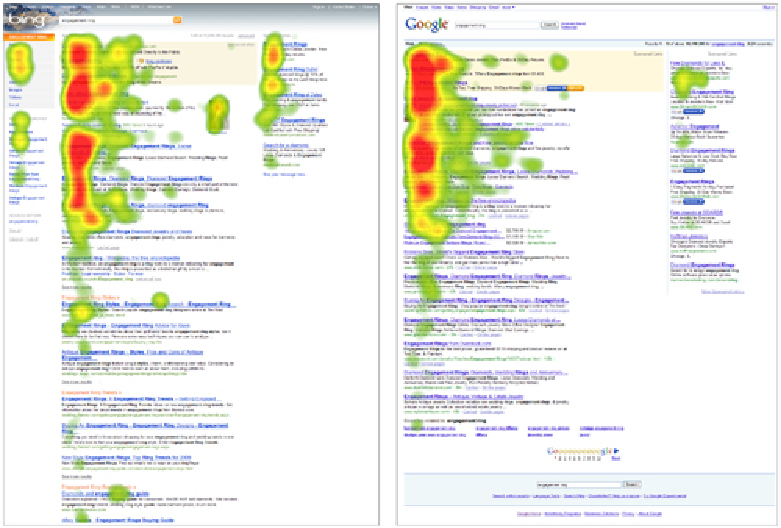
\includegraphics[width=14cm]{img/google-bing-heatmap.pdf}
	\caption{Heatmapy - vlevo Bing, vpravo Google}
	\label{img:heatmap-bing-google}
\end{figure}




%\subsubsection{Heatmapy}
%\subsubsection{Světová mapa}
%\subsubsection{Segmentace}


\subsubsection{Aplikace v praxi}

Teď, když byly nastíněny základy toho, jak webová analytika sbírá a interpretuje data je na místě se zmínit o praktickém využití těchto dat.

%Optimalizace konverze reklamních kampaní

Na počátku, kdy se měřil pouze počet zobrazení stránky, byly tyto nástroje měřítkem popularity stránek. Podle denní návštěvnosti se dalo odvodit, kolik by si měla stránka účtovat za reklamu\footnote{Dnes jsou více rozšířené sytémy, které použadují platbu za počet prokliků a jejich cena se určuje formou aukce. Například AdWords, u nás Sklik.}, většinou formou bannerů. Návštěvnost stránek i dnes určuje cenu reklamy na stránce, PR článků a obecně hodnotu celé stránky.

Když potenciální zákazník klikne na reklamu a dostane se naši stránku, stojí nás to peníze. Ne každý zákazník objedná, nebo jinak vygeneruje zisk. Takže kolik zákazníků, kteří se na naši stránku dostali přes reklamu u nás vlastně nakoupí? A ještě lépe - kolik nás ve výsledku stojí nová objednávka? Na tyto otázky standardně odpovídá napříkald Google Analytics, který je přímo napojen na AdWords\footnote{Pay Per Click reklama od Googlu}.

V okamžiku, kdy se na naši stránku dostane uživatel, vstupuje do hry měření konverze. Ta měří poměr návštěv a uskutečněných cílů - například počet objednávek, nebo počet nových emailů v seznamu odběratelů novinek. Konverzní poměr se zvlášť měří u uživatelů, kteří přišli z vyhledávače, přes reklamu anebo sami napsali adresu webové stránky do prohlížeče.

Znalost jednotlivých konverzí a napojení na reklamní systém umžňuje určit cenu za konverzi a tím i efektivitu jednotlivých kampaní.



\bigskip

%Optimalizace pro vyhledávače

Typické zdroje návštěvnosti jsou reklama, vyhledávání a dnes nově sociální média. Vyhledávače jsou kapitolou samou pro sebe. Vyhledávače používá velké denně množství lidí a je lákavé dostat svůj web do horních pozic pro vyhledávané fráze související s tématem stránky. Díky tomu, že reklama je relativně drahá je optimalizace pro vyhledávače žádanou službou, která představuje dlouhodobý nárůst návštěvnosti za jednorázovou investici.

Návštěvnost z vyhledávačů se dá efektivně měřít i s zjištěním návštěvnosti pro jednotlivé klíčové slova a vyhledávací fráze. Analytické nástoje tak umožňují změřit o kolik se zvedl počet objednávek, registrací nebo čehokoli, co majitel stránky sleduje jako cíl konverze.


%Split testing

Mocným nástrojem pro optimalizaci webových stránek je split-testování, taktéž zvané A/B testování. Tato technika spočívá v tom, že se vytvoří dvě varianty stránky a a některým uživatelům se zobrazí jedna varianta a některým druhá. Na daných stránkách se pak měří konverze a výsledkem testu je zjištění, která stránka měla větší konverzi.

Tímto způsobem se dají optimalizovat stránky, které mají zákazníka přimět k registraci, nákupu, nebo jiné cílové akci. Tato technika umožňuje určit, jaký název produktu bude mít lepší výsledky, alternativní slogany, vzhled produktu, nebo dokonce i cenu produktu. 

V případě testování ceny produktu se některým zákazníkům zobrazí například \$19 a jiným \$49. Je docela možné, že produkt za \$49 se bude lépe prodávat, protože zákazníci od něj budou očekávat větší kvalitu. Přesto, že nezní příliš sofistikovaně, umožňuje split-testing každému experimentovat s mnoha aspekty a reálně ověřit, zda navrhované změny opravdu vedou k lepší konverzi.

%optimalizace použitelnosti patří ještě pod optimalizaci konverze



Druhá strana mince je v případě webové analytiky hlubší porozumění. Do tého kategorie patří informace typu jaké prohlížeče a zařízení používají, jaký jazyk preferují, z jaké části světa jsou, odkud na stránku přicházejí, co na webu dělají a kudy stránku opouštějí. 

V závislosti na zaměřené webové stránky je tady větší nebo menší snaha poznat zákazníka. Dnešní analytcké nástroje mají pouze omezené možnosti práce se zákazníkem, především z toho důvodu, že odmítají vědět o tom, že jde o konkrétního zákazníka, jako například Google Analytics, který sledování konkrétních uživatelů přímo zakazuje v podmínkách použití.

Na práci se zákazníky se specializují jiné systémy jako jsou CRM Systémy\footnote{Customer Relationship Management systémy} a jiné úzce specializované produkty, které se již webovou analytikou nezabývají. 

Právě znalost konkrétního zákazníka a práce s ním odlišuje nový analytický produkt od ostatních. V dnešní době sodiálních médií, kdy telefonní operátoři mají teamy lidí, kteří se starají o zákaznickou podporu na sociálních sítích, je kritické mít přehled o svých zákaznících a to zvláště u webových aplikací, kde interakce zákazníka s apliakcí je to, za co nás zákazník platí.

Příští kapitola se věnuje vlastnostem nového nástroje a jejich využití.





\section{Nový nástroj}

Tato kapitola popisuje problém, který známé analytické nástroje zatím neřeší, a konkrétní způsob jeho řešení. Jak již bylo zmíněno v předchozím textu, nástroje pro webovou analytiku nepracují s konkrétními zákazníky a některé dokonce zakazují jakkoli identifikovat uživatele webů.



\subsubsection{Motivace}

%Popis problému.
Webové aplikace se od webových stránek odlišují v klíčových faktorech a tak si vyžadují odlišný náhled na analýzu jejich uživatelů. 

Asi největší rozdíl spočívá v tom, jak webové aplikace a webové stránky vydělávají peníze. U aplikace platí uživatelé za její používaní, nebo za nadstadardní služby. Menší webové stránky jako například osobní blogy většinou přímo nevydělávají, ale poskytují autorovi status profesionality a odbornosti. Ty s větší návštěvností získávají peníze pomocí reklamy, affiliate programů, nebo PR článků.

V závisloti na tom, kolik používání aplikace stojí může webová aplikace potřebovat mnohem menší množství platících uživatelů, než webová stránka neplatících návštěvníků k tomu, aby vydělávala. 

Při vývoji nové aplikace potřebují tvůrci veškerou zpětnou vazbu, kterou mohou dostat. Mají jen velmi málo uživatelů a jsou s nimi v úzkem kontaktu. Takovým uživatelům se říká "early adopters" a z hlediska vývoje je spočívá jejich úloha v používání produktu a podávání zpětné vazby. 

V okamžiku, kdy se produkt dostává k většímu počtu uživatelů, není možné se všemi udržovat písemný kontakt a jen malá část je ochotna podat zpětnou vazbu. 

V tomto okžamžiku nastupuje nový nástroj, který si klade za cíl poskytovat podporu pro práci se zákazníkem a životním cyklem zákazníků.


\subsection{Popis řešení} % co to bude umět

Životní cyklus zákazníka je možné rozdělit chronologicky do čtyř částí. Akvizice, Uživatel, Zákazník a konec využívání aplikace. Každá fáze má své specifika a vyžaduje si trochu odlišný přístup, protože nás v ní zajímá něco jiného.

\subsubsection{Akvizice uživatele}

Ještě než se z návštěvníka stane uživatel musí přijít na webovous stránku aplikace, kde se informuje o aplikaci. Většina nástrojů v této fázi dokáže identifikovat odkud uživatel přišel a dokáže říct, kolik návštěvníků z jakého zdroje se registruje.

Jelikož se konvenční nástroje omezují a unikátně neidentifikují uživatele, je tato funkce pouze jednorázová. To znamená dá se zjistit, že přes reklamní kampaň X přišlo sto návštěvníků a dva se zaregistrovali. Pokud se návštěvník na stránku vrátí a zaregistruje se až další den, nástroje to nezaznamenají kvůli anonymizaci dat.

Nový nástroj naopak pracuje s uživateli jako s lidmi, ne daty a tak každý uživatel nese informaci o tom, odkud poprvé přšel a kdy se zaregistroval. To znamená, že je možno zpětně zjistit ze kterých kampaní vzniklo nejvíce placených zákazníků globálně a ne jednorázově.

\subsubsection{Uživatel}

Když se návštěvník zaregistruje, stane se z něho uživatel. V tuto chvíli většina webových aplikací poskytuje třicetidenní testovací lhůtu, během které se uživatel má seznámit s produktem a pak se rozhodne, jestli ho bude platit, nebo ne. Tomuto způsobu se říká "trial verze".

Alternativou je tzv. Freemium, což znamená, že uživatel využívá základní verzi produktu a má možnost si zaplatit za prémiové funkce, nebo možnosti.

Narozdíl od zákazníka, který za produkt platí a tudíž se dá předpokládat, že produkt vyhovuje jeho účelům a využívá ho pro svůj prospěch není u uživatele jasná motivace. 

U trial modelu mohou uživatelé používat všechny možnosti aplikace v rámci zkušební doby, používají tedy stejnou aplikaci jako ti platící. Není však jisté, že aplikaci nepřestanou používat a začnou za ní platit. Cílem je tedy nabídnout něco, co je tak dobré, že se bez toho zákazník neobejde.

Cílem freemium modelu je nabídnout něco, co uživatelé začnou používat zdarma a časem přejdou na placenou verzi. Tento model se liší hlavně v tom, že uživatelé používají nějakým způsobem omezenou verzi. Zde se opakuje to, že není jisté, že uživatelé začnou platit, podobně jako u trial verze.

Motivace platících a neplatících uživatelů se liší. Někteří uživatelé pouze hledají možnost, jak zdarma vyřešit svůj problém a nemají zájem o prémiové funkce aplikace, jiní aplikaci jenom zkoušejí a časem si najdou jinou, nebo aplikaci sice používají, ale není pro ně tak podstatná, aby za ni platili.

Neplatící uživatelé jsou ti, kteří projevili zájem o produkt, ale ještě se nestali platícími zákazníky. U freemium modelu tato skupina početně převažuje platící uživatele zhruba 10:1 a je nutno na ní pohlížet zvlášť.

\subsubsection{Zákazník}

Zákazníci jsou ti, kteří umožňují produktu žít a rozvíjet se. Tím, že platí za produkt vyjadřují tím, že jim produkt pomáhá natolik, že jej ohodnotí svými těžce vydělanými penězi. Zákazníci jsou srdcem a duší produktu.

V dnešních webových aplikací, které hojně využívají freemium model se může jednat o pouhých 10\% všech uživatelů, často i méně. Několik procent zákazníků se v tom davu zbývajících neplatících uživatelů snadno ztratí a proto je třeba v první řadě oddělit jejich statistiky.





Z tohoto důvodu je záhodno být schopen odlišit zákazníky v analytickém nástroji a 


\subsubsection{Konec používání aplikace}






Demonstrovat na příkladu.

Popis řešení.

Co se bude měřit a proč.

Co nástroj dělá a proč.

Co nástroj nedělá a proč ne.

Pro koho je nástroj určen.

Existuje nějaký podobný nástroj?

Proč takový nástroj ještě neexistuje?
(implementujou si in house řešení tohoto problému)

\subsection{Sběr dat}

Jaké data nás zajímají a proč

Jaké data nás nezajímají a proč

Jaké jsou omezení sběru dat.

\subsection{Zpracování dat}


\subsection{Interpretace dat}

Jaké možnosti interpretace dat jsou?

Jaké možnosti se hodí?

Jaké možnosti intepretace dat jsme zvolili a proč?

Jaké jsou možnosi segmentace. 
Jaké jsou možnosti do budoucna.

Možnosti aproximace?



\subsection{Etická stránka sběru dat}

Problém etiky sběru dat.
Právní problémy.
Anonymní vs. neanonymní data.
Webaplikace vs. webová stránka.
Zákazník vs. náhodný návštěvník.
Analogie z fyzického byznysu.


Záměrné zahalování identity uživatele je argumentováno zachováním soukromí uživatele. Například Google Analytics obsahuje ve smluvním ujednání služeb Google Analytics následující text:

\begin{quote}
7.1 Nebudete slučovat (nebo nedovolíte jakékoliv třetí osobě slučování) jakákoli data shromážděná z vaší Website (vašich stránek Website) (nebo website takovéto třetí strany) s jakýmikoliv informacemi identifikujícími osoby, které pocházejí z jakéhokoli zdroje jsoucího částí vašeho užívání (nebo užívání takovéto třetí strany) Služby. Budete splňovat všechny zákony na ochranu dat a soukromí ve spojitosti s vašim používáním Služby a shromažďováním informací od návštěvníků na vašich stránkách website. Na své stránce na viditelném místě zpřístupníte (a budete i dodržovat) vhodnou směrnici o ochraně soukromí.
\ldots
\end{quote}

Na jedné straně je snaha ochránit uživatelovo soukromí, na druhé poskytnout co nejlepší službu a relevantní obsah. Etickou stránku věci se spíše zabývají velké firmy, které mají uloženo mnoho uživatelských dat a nezávislí profesionálové, kteří poukazují na přestupky a nedostatky.

Problém soukromí na webu je možno přirovnat k nakupování v obchodu. Pokud jsem v obchodním řetězci a nakupuji, budou mě sledovat kamery, které mě dokáží identifikovat a sbírají data o tom, kudy chodím. Z hlediska soukromí nechci, aby bez mého souhlasu o mě sbíral obchodní řetězec informace o tom, co nakupuji, jak často do obchodu chodím, nebo co mám na sobě. Toto je filosofie Google Analytics.

Když se svým nákupem přistoupím k pokladně, první na co se mě prodavačka zeptá je, zda mám jejich "kartu". Pokud ano, vezme si ji k zařízení napojeném na pokladnu a v tom okamžiku se můj zatím anonymní nákup stává mým nákupem a je svázán s mou kartou. Tímto způsobem obchodní řetězec dokáže sledovat jak často nakupuji a co nakupuji.

Aby měl zákazník důvod k pořízení karty, která umožňuje jeho sledování je motivován sbíráním bodů, nebo jinými výhodami\footnote{Například IKEA svým členům "IKEA Family" věnuje nápoje k jídlu zdarma.}. Při registraci pro kartu IKEA Family se do formuláře vyplňuje jméno, příjmení, bydliště, email a den narození. O ochraně osobních údajů říká IKEA, že jde o "vztah založený na důvěře". V následujícím výňatku z textu "Ochrany osobních údajů" spolešnost polopatě vysvětluje, že údaje bude poskytovat třetím stranám:

\begin{quote}
{\bf Informace, které nám sdělíte, u nás také zůstanou}\\
Kdybyste nemohli IKEA věřit, nemohli byste v ní ani nakupovat. Z toho důvodu je pro nás ochrana vašich osobních důvodů navýsost důležitá. IKEA nesděluje vaše osobní údaje jiným firmám mimo IKEA. Informace, které nám poskytnete, využívá jen a jen IKEA. Někdy sice nastanou případy, kdy Vaše osobní údaje poskytneme některé z našich divizí v jiné zemi, ale v takových případech používáme všechny dostupné administrativní, technické i fyzické způsoby ochrany dat, abychom zabránili jejich možnému prozrazení, použití, změně či zničení. Stručně řečeno se všemi dostupnými prostředky snažíme chránit vaše osobní údaje před předvídatelným nebezpečím. V některých případech však opravdu musíme některé vaše údaje sdělit jiným společnostem, které pověříme jejich zpracováním, protože od nich chceme, aby vám poskytly určité služby. Zpracování osobních údajů probíhá v těchto případech podle našich pokynů. 
\end{quote}

Velké společnosti tedy respektují naše soukromí, ale v rámci vlasntí optimalizace se nás snaží získat do svých klubů, které jim umožňují sbírat libovolná data a vyhodnocovat je.

Pro úplnost metafory o internetovém soukromí je třeba zmínit jak se k soukromí staví ti menší. Zákazník nakupuje v lahůdkářství víno a všelijaké dobroty. Lahůdkář dobře rozumí zboží a dokáže poradit a zákazník si rád nechá poradit,  protože sám není odborník a dobrou radu bere jako součást služby lahůdkářství. V této situaci nemá prodejce sepsaný dokument o ochraně osobních dat, nicméně ví, jaké zboží zákazník preferuje, jak často chodí, za kolik průměrně nakoupí a mnohdy i pro jaké příležitosti nakupuje.

To, co má lahůdkář v hlavě se ve větším měřítků nazývá Customer Relationship Management. CRM je nástroj ke shromažďování, zpracování a využití informací o zákaznících. Je to vlastně takový drobnohled, kterým se pohlíží na zákazníka jako jednotlivce. Toto kontrastuje s tím,jak data využívá firma s mnoha zákazníky, která je sohrnně analyzuje.

\bigskip

Nástroj, kterým se tato diplomová zabývá představuje řešení pro webové aplikace, které mají stovky až tisíce zákazníků, které fungují typicky na základě měsíčního předplatného. V tomto případě je potřeba kombinovat způsoby analýzy dat velkých objemů a pohledu na konkrétní zákazníky. 

Nástroj si klade za cíl podporovat webovou aplikaci od jejích začátků až k dospělosti. Zabývá se celým životním cyklem zákazníků od jejich prvního vstupu na web, přes registraci trial verze, změnu plánu na placený a používání aplikace.

V metafoře výše se je produkt na půl cesty mezi lahůdkářem, který osobně zná všechy své zákazníky a tato znalost je přidanou hodnotou služby zákazníkovi a obchodním řetězcem, který potřebuje analyzovat chování velkého množsví zákazníků.







\subsubsection{Popis technického řešení (10 Stran)}

1) diagram celého systému

2) detail sběru dat

3) detail interpretace dat

4) zobrazení dat


vizualizační technologie, appengine
proč jsem vybral tyto technologie
detaily funkce měřícího skriptu (AES)
detaily sběru dat
detaily analýzy dat






\section{Případová studie}

\subsubsection{Aplikace v reálném provozu (10 stran i s grafy)}

oběcně kolik dat tam lítalo denně, kolik uživatelů
analýza dat (na co jsem se zaměřil)
zajímavé grafy, co z nich vyplývá
závěry (navhrnout změny)

\subsubsection{Navrhnuté změny na základě získaných dat (2 stránky)}


\section{Zhodnocení}
co splnilo očekávání
co nesplnilo / předčilo očekávání
přínos pro uživatele v praxi
porovnání s podobnými nástroji




\section{Závěr}
\label{sec:Conclusion}

Nástroj splnil předpoklady..

Byla to bomba :)

\bigskip
\begin{flushright}
Michal Hantl
\end{flushright}









\begin{thebibliography}{99}


\bibitem{peci2005} Pecinovský, Rudolf,
\textit{Jak efektivně učit OOP. Tvorba softwaru 2005 – sborník přednášek}, ISBN 80-86840-14-X.

\bibitem{peci_trendy} Pecinovský, Rudolf,
\textit{Současné trendy v metodice výuky programování}, dostupné z url \url{http://gynome.nmnm.cz/konference/files/2006/sbornik/pecinovsky.pdf}.

\bibitem{plaminek} Plamínek, Jiří,
\textit{Tajemství motivace – Jak zařídit, aby pro vás lidé rádi pracovali}, ISBN 80-247-1991-6.

\bibitem{kamarati} Gašparovičová Ľuba, Hvorecký, Josef,
\textit{Kamaráti Robota Karla}, ISBN 80-06-00421-8.

\end{thebibliography}


%\appendix
%\section{Grafy a měření}
%Tohle je příloha k práci. Většinou se sem dávají grafy, tabulky, které by vzhledem
%ke svému počtu překážely v textu diplomky.
%\clearpage




\end{document}